\documentclass[11pt]{article}

\usepackage[margin=1in]{geometry}
\usepackage{amsmath,amssymb}
\usepackage{graphicx}
\usepackage{booktabs}
\usepackage{natbib}
\usepackage{hyperref}
\usepackage{xcolor}

\hypersetup{colorlinks=true, citecolor=blue, linkcolor=blue, urlcolor=blue}

\newcommand{\R}{\mathbb{R}}
\newcommand{\tr}{\operatorname{tr}}

\title{\texttt{GaussianProcessCCA}: Nonlinear Multiview Canonical\\Correlation Analysis with Gaussian-Process Encoders}

\author{
James Chapman\\
Centre for Medical Image Computing, University College London\\
\texttt{james.chapman.19@ucl.ac.uk}
}

\date{}

\begin{document}
\maketitle

\begin{abstract}
Canonical Correlation Analysis (CCA) finds linear projections of two or more views of data that are maximally correlated. Existing nonlinear extensions either require heavy machinery (deep neural encoders trained end to end) or restrict each view's encoder to be additive across features, which cannot represent genuine interactions between features of the same view. We describe \texttt{GaussianProcessCCA}, a nonlinear multiview CCA method recently added to the open-source package \texttt{cca-zoo}. Each view is encoded by a Gaussian process with a joint (non-additive) kernel over that view's raw feature vector; all views' encoders are fit jointly by minimizing an unconstrained, multiview generalization of the Eckart--Young objective rather than a per-view marginal likelihood. Writing each encoder in a fixed reduced-rank (Nystr\"om / subset-of-regressors) basis turns the fit into a smooth, exactly-gradient optimization problem solved by L-BFGS-B, with a sparse inducing-point variant that scales to thousands of samples. Because each encoder remains a Gaussian process, the method retains calibrated posterior uncertainty on every projected score at no extra cost. We describe the model, its fitting algorithm, and its complexity, and demonstrate on synthetic data that it recovers structure that is invisible to an additive nonlinear baseline and to linear ridge CCA, while its sparse approximation scales gracefully with training set size. The implementation has no dependency beyond \texttt{scikit-learn} and \texttt{scipy}, and is released as part of \texttt{cca-zoo} under the MIT license.
\end{abstract}

\section{Introduction}

Canonical Correlation Analysis \citep{hotelling1936relations} finds, for two or more views of the same set of observations, linear projections of each view that are maximally correlated with one another. It remains a workhorse tool wherever multiple measurement modalities are collected on the same units --- neuroimaging and genetics \citep{bach2005probabilistic,klami2013bayesian}, multilingual text, and multi-sensor signals. Linear CCA, however, can only recover correlated structure that is itself linear in the raw features, which motivated a long line of nonlinear extensions: kernel CCA \citep{hardoon2004canonical}, which implicitly maps each view through a fixed nonlinear feature map and is exact but scales cubically in sample count with no obvious route to out-of-sample uncertainty; and deep CCA \citep{andrew2013deep,wang2015deep}, which replaces each view's encoder with a neural network trained by stochastic gradient descent, at the cost of substantial architecture and optimization tuning and the loss of any probabilistic interpretation of the learned projection.

The \texttt{cca-zoo} package \citep{chapman2021cca} already offers a lighter-weight nonlinear alternative, \texttt{GAMCCA}, which represents each view's encoder as a sum of univariate B-splines --- a generalized additive model \citep{hastie1999generalized} --- fit against the same shared multiview objective used throughout the package. An additive encoder is cheap and interpretable, but by construction cannot represent an interaction between two features of the same view (e.g. a latent factor that depends on $x_1 x_2$ rather than on $x_1$ and $x_2$ separately): no sum of one-dimensional functions of $x_1$ and of $x_2$ can express $x_1 x_2$.

This note describes \texttt{GaussianProcessCCA}, added to \texttt{cca-zoo} to close this gap. Each view's encoder is a Gaussian process (GP) with a joint kernel over that view's entire raw feature vector, so it represents feature interactions directly rather than approximating them through an ensemble of additive or tree-based splits. Unlike a textbook GP regression model, however, the encoders here are not fit against a per-view target and marginal likelihood: all views' GPs are fit jointly, directly against the same unconstrained multiview CCA objective used by every other model in \texttt{cca-zoo}. The result keeps three properties that matter in practice: (i) it represents genuine cross-feature interactions that additive nonlinear CCA cannot; (ii) it remains a Gaussian process, so every projected score comes with a calibrated posterior standard deviation, essentially for free; and (iii) it introduces no new dependency --- the entire method is built from \texttt{scikit-learn}'s existing \texttt{GaussianProcessRegressor}, kernel, and clustering primitives, plus \texttt{scipy.optimize}.

\section{Background: the unconstrained (Eckart--Young) CCA objective}
\label{sec:ey}

\texttt{GaussianProcessCCA} reuses the same training objective as several other nonlinear models already in \texttt{cca-zoo} (\texttt{CCAEY}, \texttt{DCCAEY}, \texttt{TreeCCA}, \texttt{GAMCCA}), introduced by \citet{chapman2024unconstrained} as an unconstrained, stochastic-optimization-friendly surrogate for classical CCA. For $M$ views with embeddings $Z_1,\dots,Z_M \in \R^{n\times k}$ produced by per-view encoders $f_i$, define the mean pairwise cross-covariance (summed over \emph{all} ordered pairs, including $i=j$) and the mean auto-covariance,
\[
C = \frac1M \sum_{i,j} \operatorname{Cov}(Z_i, Z_j), \qquad V = \frac1M \sum_i \operatorname{Cov}(Z_i, Z_i).
\]
The Eckart--Young (EY) loss to be minimized over the encoders is
\begin{equation}
\mathcal{L}_{EY}(Z_1,\dots,Z_M) = -2\,\tr(C) + \tr(VV).
\label{eq:ey}
\end{equation}
The first term rewards embeddings that covary strongly across views; the second penalizes each view's own embedding from drifting away from an (approximately) whitened, unit-scale representation, which prevents the trivial solution of scaling $Z_i$ to infinity. Unlike the classical CCA generalized eigenvalue problem, \eqref{eq:ey} is an ordinary unconstrained smooth objective in the entries of $Z_1,\dots,Z_M$, with a simple closed-form gradient with respect to any one view's embedding \citep{chapman2024unconstrained}. This is what lets \texttt{cca-zoo} plug in encoders as different as linear projections, deep networks, gradient-boosted trees, splines, or --- here --- Gaussian processes, and fit all of them by ordinary gradient-based optimization rather than by an eigendecomposition or a bespoke per-model algorithm.

\section{Method}

\subsection{Per-view encoder: a reduced-rank Gaussian process}
\label{sec:encoder}

For view $i$ with training data $X_i \in \R^{n\times p_i}$, \texttt{GaussianProcessCCA} fixes a kernel $k$ (an ARD RBF kernel by default, with one lengthscale per feature) and a set of $m$ basis points $Z_i \in \R^{m \times p_i}$ --- every training row when $m \ge n$ (\emph{exact} inference), or $m = \texttt{n\_inducing}$ rows chosen by \texttt{k-means++} seeding \citep{quinonero2005unifying} when a smaller $m$ is requested (\emph{sparse} inference). The encoder is written in the standard Nystr\"om / subset-of-regressors reduced-rank form \citep{williams2001using,quinonero2005unifying},
\begin{equation}
f_i(x) = k(x, Z_i)^\top B_i, \qquad B_i \in \R^{m \times k},
\label{eq:encoder}
\end{equation}
for learnable coefficients $B_i$. The cross-kernel $k(X_i, Z_i)$ is centered with a \texttt{KernelCenterer} fit on the inducing-point Gram matrix $K_{mm} = k(Z_i, Z_i)$ --- the same double-centering used by kernel PCA --- which makes $f_i$ automatically zero-mean for \emph{any} $B_i$, so no separate re-centering step is needed downstream. Only the coefficients $B_i$ are learned; the kernel's own hyperparameters (lengthscales, signal variance) are fixed by the user (or left at their ARD-RBF default) rather than tuned by marginal-likelihood optimization, since the model already has one other set of parameters to optimize per view and, unlike ordinary GP regression, has no single scalar target to define a marginal likelihood against.

\subsection{Joint fitting: penalized EY loss by block-coordinate L-BFGS-B}

Because \eqref{eq:encoder} is linear in $B_i$ given the fixed basis $k(X_i, Z_i)$, substituting it into the multiview objective \eqref{eq:ey} plus an RKHS-norm ridge penalty gives, for view $i$ with every other view's embedding held fixed,
\begin{equation}
\mathcal{L}(B_i) = \mathcal{L}_{EY}(Z_1, \dots, Z_M) + \frac{\alpha}{2}\sum_{c=1}^k B_i[:,c]^\top K_{mm}\, B_i[:,c],
\label{eq:penalized}
\end{equation}
an ordinary smooth function of $B_i$ with an exact analytic gradient obtained by the chain rule through \eqref{eq:encoder} and the known gradient of $\mathcal{L}_{EY}$ \citep{chapman2024unconstrained}:
\begin{equation}
\nabla_{B_i}\mathcal{L} = k(X_i, Z_i)^\top \nabla_{Z_i}\mathcal{L}_{EY} + \alpha\, K_{mm}\, B_i.
\label{eq:grad}
\end{equation}
The penalty in \eqref{eq:penalized} is the RKHS squared norm a Gaussian process's own posterior mean minimizes -- not a plain $\lVert B_i\rVert_2^2$, which would ignore the kernel's geometry entirely.

All views' coefficients are fit by cycling through views in a block Gauss--Seidel scheme: at each sweep, every view's full coefficient matrix $B_i$ is optimized to convergence by L-BFGS-B (using \eqref{eq:penalized}--\eqref{eq:grad} directly, so no explicit Hessian is needed) with every other view's embedding held fixed, and sweeps repeat until the penalized objective changes by less than a tolerance $\texttt{tol}$ between consecutive sweeps or a maximum number of sweeps $\texttt{max\_iter}$ is reached. Coefficients are initialized from a cheap random-projection whitening of each view's own basis. This is the same L-BFGS-B routine \texttt{scikit-learn}'s own \texttt{GaussianProcessRegressor} uses internally for its marginal-likelihood optimization, just pointed at a different objective.

\subsection{Predictive uncertainty}

Because each encoder is a Gaussian process, \texttt{GaussianProcessCCA} retains calibrated predictive uncertainty on its projections without any extra modeling effort. The posterior variance of a GP's predictive mean is a standard closed-form expression involving only the kernel, the noise level, and the design points -- never the fitted targets -- so it does not depend on $B_i$ at all. The implementation exploits this directly: alongside the centered basis used to fit the mean, each view also holds an ordinary \texttt{GaussianProcessRegressor} fit on the (uncentered) inducing points with a placeholder all-zero target and no hyperparameter optimization; only its closed-form predictive standard deviation is ever used. Calling \texttt{transform(..., return\_std=True)} therefore returns, alongside each view's projected mean, a posterior standard deviation per latent dimension that grows away from the training data and shrinks near it, exactly as for any other GP posterior.

\subsection{Complexity}

Exact and sparse inference are the same reduced-rank construction, differing only in how many basis points are used: $m = n$ for exact inference, or $m = \texttt{n\_inducing} < n$ chosen by \texttt{k-means++} for the sparse approximation. Since forming the basis and its Gram matrix costs $O(nm^2 + m^3)$ and every subsequent L-BFGS-B iteration is a small number of matrix-vector products of the same order, fitting scales as $O(nm^2 + m^3)$ overall -- cubic in $n$ for exact inference, and linear in $n$ once the number of inducing points $m \ll n$ is fixed, letting the sparse variant scale to training sets of several thousand samples where exact inference is impractical.

\subsection{Software}

\texttt{GaussianProcessCCA} is implemented entirely on top of existing \texttt{scikit-learn} \citep{pedregosa2011scikit} building blocks -- \texttt{GaussianProcessRegressor}, \texttt{RBF}, \texttt{ConstantKernel}, \texttt{KernelCenterer}, and \texttt{kmeans\_plusplus} -- with \texttt{scipy.optimize.minimize} performing the fit, so it introduces no new required dependency beyond what \texttt{cca-zoo} already requires. It follows the same \texttt{scikit-learn}-style \texttt{fit}/\texttt{transform}/\texttt{score} API as every other model in \texttt{cca-zoo}:
\begin{verbatim}
from cca_zoo.gp import GaussianProcessCCA

model = GaussianProcessCCA(latent_dimensions=1, n_inducing=200)
model.fit([X1, X2])
z1, z2 = model.transform([X1, X2])
(mean1, mean2), (std1, std2) = model.transform([X1, X2], return_std=True)
corrs = model.score([X1, X2])
\end{verbatim}
It supports two or more views, and is released as free and open-source software under the MIT license as part of \texttt{cca-zoo}.\footnote{\url{https://github.com/jameschapman19/cca_zoo}}

\section{Related work}

Kernel CCA \citep{hardoon2004canonical} also encodes each view through a fixed, joint (non-additive) kernel, and is in this sense the closest classical relative of \texttt{GaussianProcessCCA}; the two differ in how coefficients are fit (kernel CCA solves a generalized eigenvalue problem in the dual, rather than minimizing \eqref{eq:penalized} by gradient-based optimization) and in that kernel CCA carries no notion of predictive uncertainty. Probabilistic and Bayesian CCA \citep{bach2005probabilistic,klami2013bayesian} instead place a linear-Gaussian generative model over a \emph{shared} latent variable that is common to all views, giving uncertainty over that shared factor; \texttt{GaussianProcessCCA} instead keeps the multiview EY training objective and per-view encoders of \texttt{cca-zoo}'s other models, and its posterior uncertainty is over each per-view encoder's output, not a shared latent factor. Gaussian process latent variable models \citep{lawrence2005probabilistic} and their multi-view extensions such as manifold relevance determination \citep{damianou2012manifold} likewise place a GP prior over a shared latent space and infer it by maximizing a marginal likelihood; \texttt{GaussianProcessCCA} instead fits per-view GP \emph{encoders} against the discriminative EY objective shared with the rest of \texttt{cca-zoo}, which is considerably simpler to optimize (ordinary L-BFGS-B on a closed-form objective and gradient) at the cost of the fully Bayesian treatment of the latent space that a GP-LVM provides. On the sparse-approximation side, the reduced-rank construction used here is the same subset-of-regressors / Nystr\"om approximation surveyed by \citet{quinonero2005unifying} and used, in different forms, by \citet{snelson2006sparse} and \citet{titsias2009variational}; unlike the latter's variational treatment, inducing points here are chosen once by \texttt{k-means++} clustering rather than optimized, which keeps the fitting problem an ordinary (non-variational) smooth optimization at the cost of a somewhat less tight approximation to the exact posterior. Within \texttt{cca-zoo} itself, \texttt{GaussianProcessCCA} sits alongside \texttt{GAMCCA} (additive splines) and \texttt{TreeCCA} (gradient-boosted trees) as a third nonlinear encoder choice, trading \texttt{GAMCCA}'s interpretability and speed for the ability to represent joint feature interactions directly.

\section{Experiments}
\label{sec:experiments}

Both experiments below use synthetic data so that the ground-truth correlated structure is known; code to reproduce both figures is included with the paper source.

\subsection{Recovering a genuine feature interaction}

We construct two views of $n$ samples each. View 1 consists of two independent standard normal factors $u, v$ (plus noise); view 2 is two noisy copies of their \emph{interaction} $u v$, which is not separable into a function of $u$ plus a function of $v$. We compare \texttt{GaussianProcessCCA} (default ARD-RBF kernel, exact inference) against linear \texttt{rCCA}, additive \texttt{GAMCCA}, and gradient-boosted-tree \texttt{TreeCCA} \citep{chen2016xgboost}, all at a single latent dimension, training on $300$ samples and reporting the canonical correlation on $300$ held-out samples, averaged over 10 random seeds (Figure~\ref{fig:interaction}; error bars are one standard deviation across seeds). Linear \texttt{rCCA} recovers nothing ($0.005 \pm 0.097$), as expected: $u$ and $v$ are independent and mean zero, so $uv$ is linearly uncorrelated with either. \texttt{TreeCCA} at its default settings likewise averages to essentially zero, with high seed-to-seed variance ($-0.003 \pm 0.123$): at \texttt{colsample\_bytree}'s default subsampling rate, individual trees are frequently built from only one of view 1's two features, so a single boosted tree only rarely sees both $u$ and $v$ in a single split path and cannot reliably fit their interaction. \texttt{GAMCCA} recovers substantial but incomplete correlation ($0.825 \pm 0.011$): although no sum of one-dimensional functions of $u$ and $v$ can correlate with the \emph{signed} product $uv$ itself (for independent, mean-zero $u,v$, $\operatorname{Cov}(f(u)+g(v), uv)=0$ for any $f,g$), an additive encoder can still correlate with an \emph{even} transformation of the interaction that its partner view is free to fit instead --- e.g.\ $\operatorname{Cov}(u^2+v^2,\, u^2v^2) = 4 \neq 0$ for standard normal $u,v$, since $u^2+v^2$ and $|uv|$ are positively associated. \texttt{GaussianProcessCCA}'s joint (non-additive) kernel is not restricted to this even/energy-like proxy and represents the signed interaction directly, recovering the highest held-out correlation of the four ($0.889 \pm 0.019$).

\begin{figure}[t]
\centering
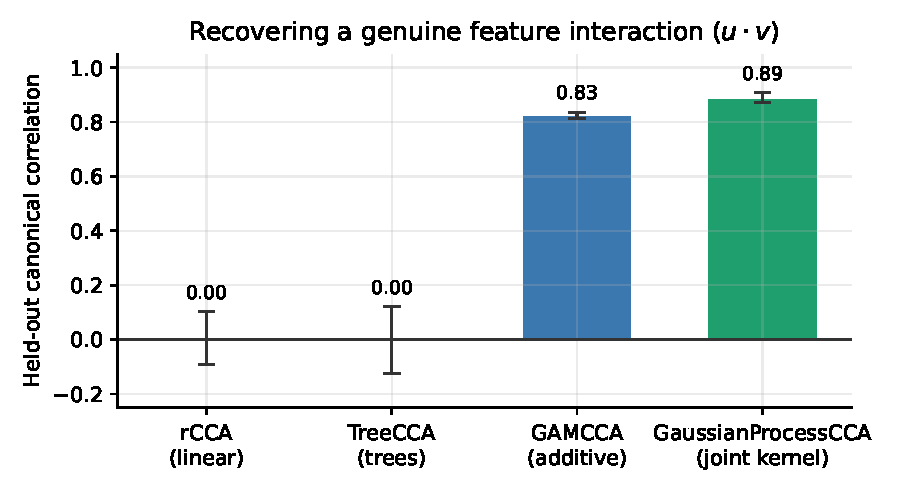
\includegraphics[width=0.85\textwidth]{fig1_interaction.pdf}
\caption{Held-out canonical correlation on the feature-interaction task (Section~\ref{sec:experiments}), mean $\pm$ one standard deviation over 10 seeds. \texttt{GaussianProcessCCA}'s joint, non-additive kernel recovers the signed $uv$ interaction most fully; additive \texttt{GAMCCA} recovers only a partial, sign-blind proxy; linear \texttt{rCCA} and default-settings \texttt{TreeCCA} recover essentially nothing.}
\label{fig:interaction}
\end{figure}

\subsection{Scaling with the sparse approximation}

We next construct two views of $n=4500$ samples sharing a nonlinear latent factor ($X_2$ driven by the square of the same latent $z$ that drives $X_1$), and fit \texttt{GaussianProcessCCA} with \texttt{n\_inducing} $\in \{20, 50, 100, 200, 400\}$ on $4000$ training samples, reporting held-out canonical correlation on $500$ test samples and wall-clock fit time for each setting (Figure~\ref{fig:scaling}), against exact inference on a subsample of $800$ training points (the largest exact fit we ran within this paper's compute budget, since exact inference is $O(n^3)$: it already takes $74.7$s on $800$ points, longer than any sparse setting tried here on $5\times$ as much training data). Held-out correlation rises from $0.929$ at \texttt{n\_inducing}$=20$ to $0.934$ by \texttt{n\_inducing}$=100$ and is essentially flat thereafter (up to $0.934$ at \texttt{n\_inducing}$=400$), matching the $0.929$ held-out correlation of exact inference on the $800$-point subsample. Fit time grows with \texttt{n\_inducing} (from $0.9$s at $20$ inducing points to $55$s at $200$--$400$), consistent with the $O(nm^2+m^3)$ scaling of Section~\ref{sec:encoder}, but a moderate \texttt{n\_inducing} already captures essentially all of the achievable held-out correlation: the sparse approximation matches exact inference's held-out quality on $5\times$ more training data, at a comparable or lower fit cost.

\begin{figure}[t]
\centering
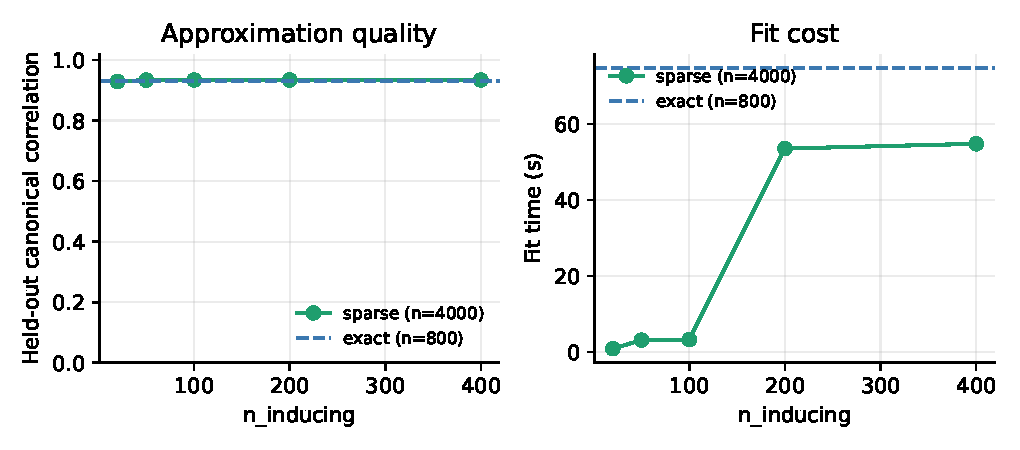
\includegraphics[width=0.85\textwidth]{fig2_scaling.pdf}
\caption{Sparse \texttt{GaussianProcessCCA} on $n=4000$ training samples: held-out canonical correlation and fit time as a function of the number of inducing points, against exact inference on a subsample of $800$ points (the largest exact fit run for this paper; exact inference is $O(n^3)$ and does not scale to the full $4000$-sample training set within a similar compute budget).}
\label{fig:scaling}
\end{figure}

\section{Limitations}

Kernel hyperparameters (lengthscales, signal variance) are fixed rather than tuned automatically by marginal-likelihood optimization; the user either supplies a kernel directly or tunes it externally (e.g.\ with \texttt{scikit-learn}'s \texttt{GridSearchCV}, since \texttt{GaussianProcessCCA} is an ordinary \texttt{BaseEstimator}). Exact inference remains $O(n^3)$, so datasets beyond a few thousand samples require the sparse approximation, whose inducing points are selected once by \texttt{k-means++} clustering rather than jointly optimized with the coefficients. Finally, because the encoder is a joint kernel over each view's raw features rather than a linear map or a sum of per-feature terms, \texttt{GaussianProcessCCA} has no per-feature loading matrix or additive shape function to inspect, unlike \texttt{cca-zoo}'s linear and \texttt{GAMCCA} models -- interpretability is traded for the ability to represent feature interactions.

\section{Conclusion}

\texttt{GaussianProcessCCA} adds a nonlinear multiview CCA model to \texttt{cca-zoo} that represents genuine cross-feature interactions within a view -- something the package's existing additive (\texttt{GAMCCA}) and tree-based (\texttt{TreeCCA}) nonlinear models cannot do directly -- while remaining a Gaussian process, so every projected score comes with calibrated predictive uncertainty. Writing each view's encoder in a fixed reduced-rank kernel basis reduces fitting to an ordinary smooth optimization problem, solved by L-BFGS-B against the same unconstrained multiview objective used throughout \texttt{cca-zoo}, with a sparse inducing-point variant that scales to several thousand samples. The method is implemented entirely on existing \texttt{scikit-learn} primitives and released under the MIT license.

\bibliographystyle{plainnat}
\bibliography{paper}

\end{document}
